\chapter{Η συνεισφορά μας}

Στο κεφάλαιο αυτό αναλύεται η δική μας συνεισφορά και τα πειράματα μας. Αρχικά, περιγράφονται αναλυτικά τo διαλογικό σύστημα \en{Rasa}, καθώς και το σύστημα ενισχυτικής μάθησης \en{Vowpal Wabbit}. Έπειτα, περιγράφεται η διαδικασία που ακολουθήσαμε, καθώς και τα προβλήματα που ανέκυψαν κατά την διαδικασία. Τέλος περιγράφεται η πλήρης αρχιτεκτονική του συστήματος και η λειτουργία του.

\section{Το διαλογικό σύστημα \en{Rasa}}

Το \en{Rasa} είναι ένα πλαίσιο (\en{framework}) ανοιχτού κώδικα για την ανάπτυξη και την έκδοση εφαρμογών συνομιλίας τεχνητής νοημοσύνης. Παρέχει ένα σύνολο εργαλείων και βιβλιοθηκών που επιτρέπουν στους προγραμματιστές να δημιουργούν διαλογικούς πράκτορες, εικονικούς βοηθούς και άλλους συνομιλητές. Το \en{Rasa} έχει σχεδιαστεί για να προσφέρει ευελιξία και έλεγχο της συμπεριφοράς και των δυνατοτήτων αυτών των συστημάτων τεχνητής νοημοσύνης.

Το πλαίσιο \en{Rasa} μπορεί νοητικά να χωριστεί σε δύο κομματια. Τα κομμάτια αυτά στο παρελθόν ήταν και ξεχωριστές υπηρεσίες, αλλά πλέον όλα βρίσκονται σε ένα πακέτο: το \en{Rasa NLU (Natural Language Understanding)} υπεύθυνο για την κατανόηση φυσικής γλώσσας και το \en{Rasa Core}.

To \en{Rasa NLU} είναι υπεύθυνο για την κατανόηση των εισροών των χρηστών και την εξαγωγή σχετικών πληροφοριών από αυτές. Χρησιμοποιεί τεχνικές μηχανικής μάθησης για την επεξεργασία και την ταξινόμηση των μηνυμάτων των χρηστών, εξάγοντας οντότητες και προθέσεις.

Το \en{Rasa Core} χειρίζεται τη διαχείριση του διαλόγου και τη διαδικασία λήψης αποφάσεων. Χρησιμοποιεί ενισχυτική μάθηση για να εκπαιδεύσει μοντέλα που μπορούν να προβλέψουν την επόμενη καλύτερη ενέργεια με βάση την τρέχουσα κατάσταση της συνομιλίας. Το \en{Rasa Core} επιτρέπει στους προγραμματιστές να ορίζουν τις ροές συνομιλιών, να χειρίζονται τις απαντήσεις των χρηστών και να διαχειρίζονται το περιβάλλον και την κατάσταση.

Ένα από τα βασικά πλεονεκτήματα του \en{Rasa} είναι η ευελιξία και η δυνατότητα προσαρμογής του. Οι προγραμματιστές μπορούν να ορίσουν τα δικά τους μοντέλα γλώσσας για συγκεκριμένο τομέα, να τους εκπαιδεύσουν χρησιμοποιώντας τα δικά τους δεδομένα και να τα βελτιστοποιήσουν για να επιτύχουν καλύτερη απόδοση. Το \en{Rasa} υποστηρίζει επίσης την ενοποίηση με άλλες υπηρεσίες και πλατφόρμες, επιτρέποντας στους προγραμματιστές να συνδέουν τους διαλογικούς τους πράκτορες τους με διάφορα κανάλια, όπως ιστότοπους, εφαρμογές ανταλλαγής μηνυμάτων και φωνητικές διεπαφές.

To \en{Rasa} βασίζεται στην ιδέα της ανάπτυξης βασισμένης στις συνομιλίες (\en{Conversation Driver Development}). Αυτό σημαίνει ότι η καλύτερη πηγή πληροφορίας για την βελτίωση του διαλογικού πράκτορα προέρχεται από τις πραγματικές συνομιλίες που δημιουργούνται από την επικοινωνία με χρήστες.

Αν και αρχικά το \en{Rasa} χρησιμοποιούσε σε μεγάλο βαθμό την ιδέα των προθέσεων για την δημιουργία των πρακτόρων, τον τελευταίο καιρό έχουν αρχίσει να δοκιμάζουν να χτίσουν εργαλεία, τα οποία θα επιτρέψουν στους πράκτορες να λειτουργήσουν χωρίς προθέσεις, δημιουργώντας ένα σύστημα άκρη-σε-άκρη (\en{end-to-end}), στο οποίο το σύστημα διαχείρισης του διαλόγου θα χρησιμοποιεί το κείμενο της απάντησης για να επιλέξει την επόμενη κατάσταση του διαλόγου, αντί να βασίζεται στην πρόθεση, όπως φαίνεται στο Σχήμα~\ref{fig:rasa_intentless}. Φυσικά, αυτό δεν σημαίνει ότι οι προθέσεις δεν έχουν χρήση, αλλά σε περιπτώσεις που το σύστημα δεν μπορεί με μεγάλη βεβαιότητα να προβλέψει την πρόθεση, η χρήση της πολιτικής χωρίς προθέσεις μπορεί να φέρει καλύτερα αποτελέσματα.

\begin{figure}
    \centering
    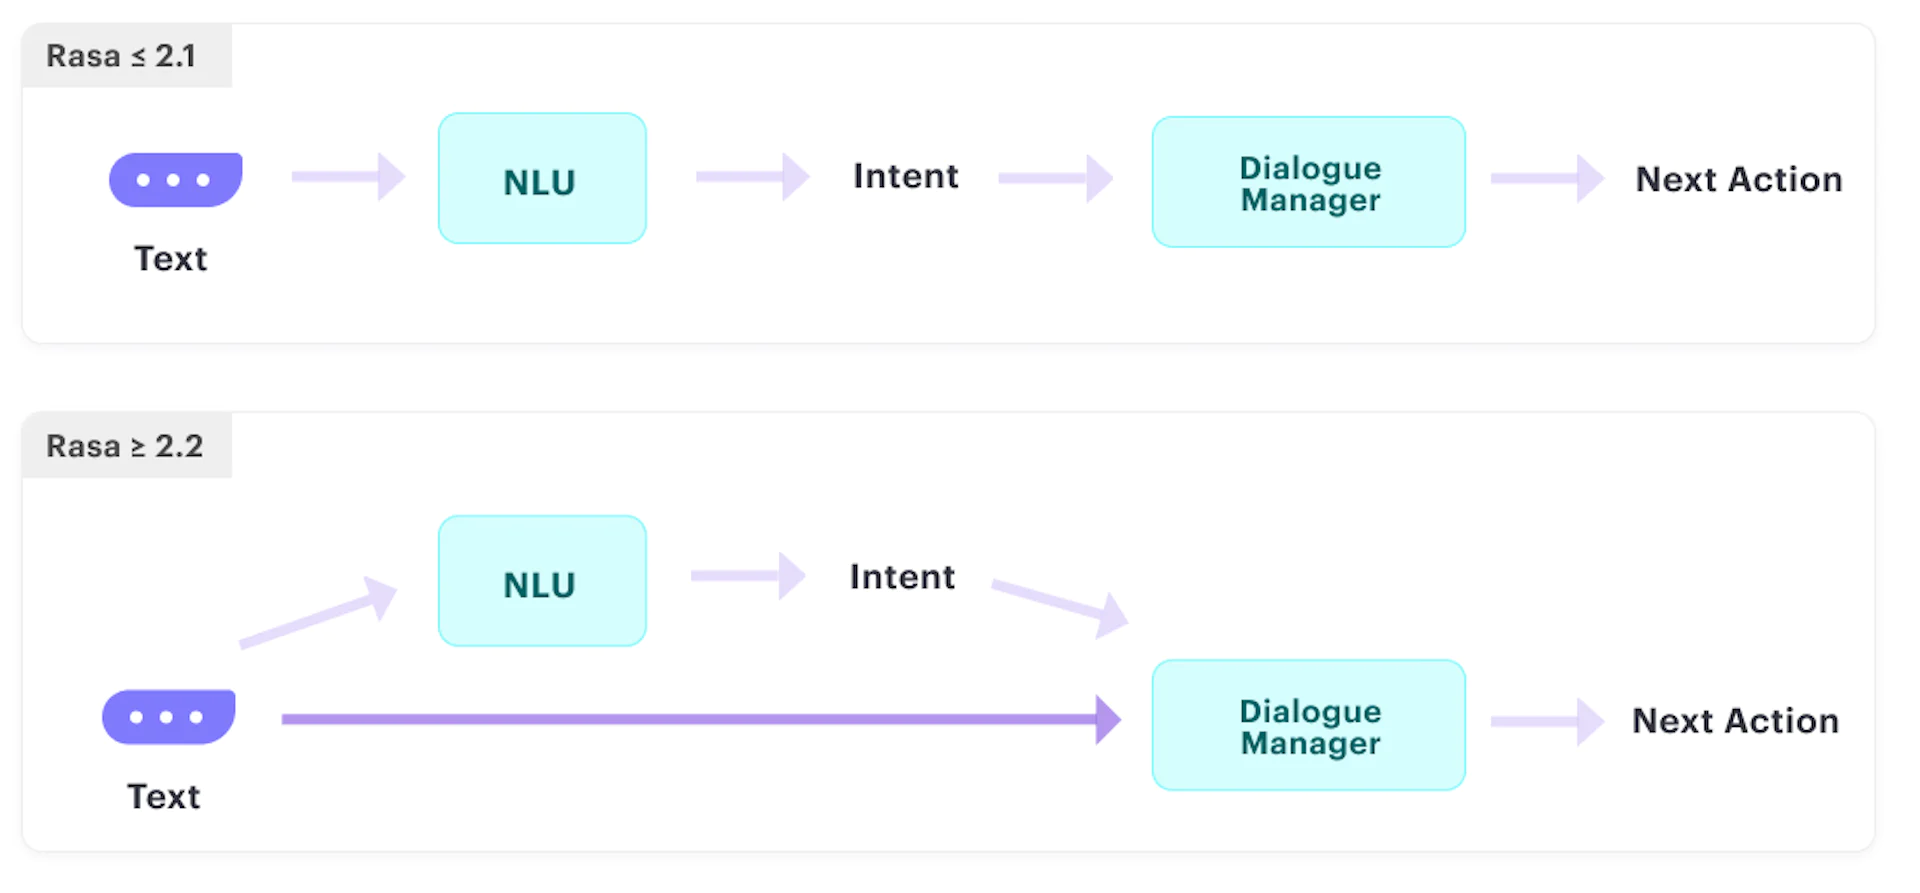
\includegraphics[width=\textwidth]{body_matter/our_work/images/rasa_intentless.png}
    \caption{Η αρχιτεκτονική του συστήματος με και χωρίς προθέσεις}
    \label{fig:rasa_intentless}
\end{figure}


\subsection{\en{Rasa NLU}}

Το \en{Rasa NLU} είναι το κομμάτι της εφαρμογής υπευθυνο για την κατανόηση της φυσικής γλώσσας. Το \en{Rasa} χρησιμοποιεί μια τεχνική η οποία ονομάζεται \en{DIET (Dual Intent and Entity Transformer)}, το οποίο είχε καλύτερα αποτελέσματα από \en{fine-tuning} ενός μοντέλου \en{BERT}, μετασχηματιστή που το 2020 θεωρούνταν τελευταίας τεχνολογίας. Το \en{DIET} έχει διττό ρόλο, καθώς διαχειρίζεται τόσο την αναγνώριση των προθέσεων, όσο και την εξαγωγή προθέσεων. H αρχιτεκτονική του \en{DIET} φαίνεται στο Σχήμα~\ref{fig:diet_architecture}.

Η δομή του μοντέλου είναι η εξής. Έστω ότι, για παράδειγμα, ο χρήστης λέει \en{"play ping pong"}, οταν ο πράκτορας τον ρωτήσει τι θα ήθελε να κάνει. Η πρόταση θα σπάσει σε λέξεις (\en{tokens}), και κάθε μια θα περάσει μέσα από ένα κομμάτι του δικτύου με δύο διαδρομές. Η πρώτη είναι η προ-εκπαιδευμένη διαδρομή, κάτα την οποία η λέξη περνάει μέσα από ένα προ-εκπαιδευμένο δίκτυο και επιστρέφει μια διανυσματική αναπαράσταση της λέξης. Αυτό το δίκτυο μπορεί να είναι κάποιος μετασχηματιστής για παράδειγμα. Η άλλη διαδρομή μετατρέπει πρώτα την λέξη σε μια αραιή αναπαράσταση της με βάση τις λέξεις και τα \en{n-grams} που δημιουργούνται και μετά περνάει μέσα από ένα νευρωνικό δίκτυο, κάνοντας την πράξη $g(Wx + b)$, όπου $x$ είναι η αραιή αναπαράσταση, $W$ τα βάρη του δικτύου και $b$ η κλίση (\en{bias}). Έπειτα τα δύο διανύσματα από τις δύο διαδρομές ενώνονται και περνάνε μέσα από ένα ακόμα νευρωνικό δίκτυο, το οποίο έχει ως έξοδο ένα διανυσμα 256 διαστάσεων. Τα νευρωνικά δίκτυα αυτά δεν είναι πλήρως συνδεδεμένα, αλλά έχουν αφαιρεθεί κάποιες ακμές με χρήση \en{drop-out}. Επιπλέον όλα τα νευρωνικά δίκτυα που βρίσκονται στο ίδιο επίπεδο, έχουν τα ίδια βάρη.

Πέρα από τις λέξεις, στο σύστημα εισέρχεται και το \en{\texttt{\_\_CLS\_\_} token}, το οποίο ουσιαστικά είναι η αναπαράσταση ολόκληρης της πρότασης. Αυτή η αναπαράσταση ουσιαστικά δημιουργείται είτε με την ένωση των διανυσμάτων των επιμέρους λέξεων, στο κομμάτι της δημιουργίας της αραιής αναπαράστασης είτε είναι η αναπαράσταση της πρότασης μέσα από το προ-εκπαιδευμένο δίκτυο.

Ακόμα, κατα την εκπαίδευση, μια από τις λέξεις συγκαλύπτεται με μια μάσκα, το \en{\texttt{\_\_MASK\_\_}}. Στο παράδειγμα του Σχήματος~\ref{fig:diet_architecture}, η λέξη αυτή είναι το \en{pong}. Αυτή η λέξη μετά θα πρέπει να προβλεφθεί από τον μετασχηματιστή. Αυτη η πρόβλεψη θα περάσει μετά από ενα δίκτυο διανυσματικής αναπαράστασης και θα συγκριθεί με την πραγματική λέξη. Αυτό μας δείχνει πόσο καλά το μοντέλο μας μπορεί να γενικεύσει την γλώσσα.

Ακόμα, κατά την εκπαίδευση, μια παρόμοια διαδικασία συμβαίνει μεταξύ του \en{\texttt{\_\_CLS\_\_} token} και της (γνωστής) πρόθεσης του χρήστη, καθώς στηριζόμαστε στην ιδέα ότι το \en{token}, αφού αναπαριστά ολόκληρη την πρόταση, φέρει πληροφορία σχετικά με την πρόθεση.

Τέλος, οι λέξεις αφού περάσουν μέσα από τον μετασχηματιστή, συγκρίνονται με τις πραγματικές οντότητες που αναπαριστούν μέσα σε ένα υπό συνθήκη τυχαίο πεδίο (\en{Conditional Random Field}) και υπολογίζεται μια απώλεια.

Έτσι το σύστημα ολόκληρο εκπαιδεύεται με βάση την συνολική απώλεια που προκύπτει από το σφάλμα στην αναγνώριση οντοτήτων, στην πρόβλεψη της λέξης μέσα στην πρόταση και την κατανοηση της πρόθεσης του χρήστη.
\begin{figure}
    \centering
    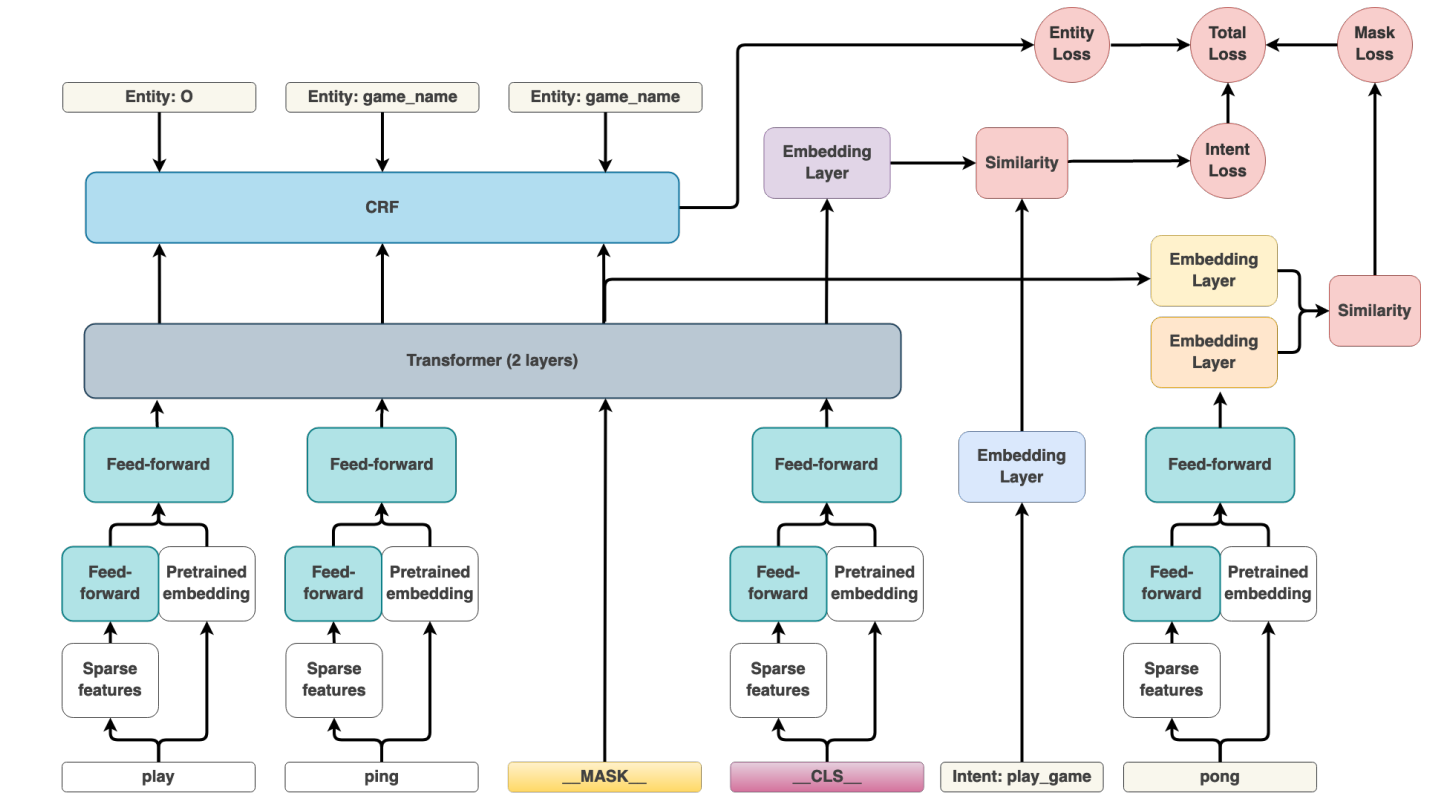
\includegraphics[width=\textwidth]{body_matter/our_work/images/DIET_architecture.png}
    \caption{Η αρχιτεκτονική του συστήματος \en{DIET}\cite{bunk2020diet}}
    \label{fig:diet_architecture}
\end{figure}

\subsection{\en{Rasa Core}}

Στο κομμάτι αυτό γίνεται η διαχείριση του διαλόγου και η επιλογή της επόμενης κίνησης. Ακόμα γίνεται η παραγωγή του διαλόγου. Θα εξηγήσουμε περιληπτικά το πώς λειτουργούν τα μέρη αυτά.

Το \en{Rasa} χρησιμοποιεί ένα σύνολο από πολιτικές για την διαχείριση του διαλόγου, και ανάλογα με την προτεραιότητα τους και την εμπιστοσύνη που έχουν στην πρόβλεψη τους, επιλέγει ποια θα χρησιμοποιήσει.

Μια από τις πιο σημαντικές είναι η πολιτική \en{TED (Transformer Embedding Dialogue)}.Η πολιτική \en{TED} χρησιμοποιείται για την επιλογή της επόμενης ενέργειας και την αναγνώριση οντοτήτων. Για την επιλογή της ενέργειας, η πολιτική ενώνει σε ένα διάνυσμα την αναπαράσταση της προηγούμενης πράξης, της πρόθεσης και πληροφοριών που είναι απαραίτητο να είναι διαθέσιμες μακροχρόνια (όπως πληροφορίες από κάποια φόρμα). Έπειτα, αυτές περνάνε μέσα από ένα μετασχηματιστή, παρέα με τις αναπαραστάσεις των προηγούμενων καταστάσεων. Η έξοδος του μετασχηματιστή περνάει μέσα από ένα νευρωνικό δίκτυο όπου γίνεται η πρόβλεψη της πρότασης που θα κάνει το σύστημα, μαζί με μια βεβαιότητα στην πρόταση αυτή.

Με αυτό τον τρόπο, το σύστημα μπορεί να διαχειριστεί την επικοινωνία με τον χρήστη όταν αυτός ξεφεύγει από το χαρούμενο μονοπάτι και μπορεί να επιστρέψει στην αρχική συζήτηση. Για την εκπαίδευση αυτού του συστήματος, χρησιμοποιούνται δεδομένα, τα οποία λέγονται ιστορίες (\en{stories}). Οι ιστορίες αυτές περιγράφουν τα διαλογικά μονοπάτια των χρηστών, και είναι η βάση της ανάπτυξης με βάση την συνομιλία. Καθώς οι χρήστες χρησιμοποιούν τον διαλογικό πράκτορα και κάνουν συζητήσεις μαζί του, οι προγραμματιστές μπορούν να αναγνωρίσουν ποια ειναι τα πιο συχνά καλά ή κακά μονοπάτια που παίρνουν και να τα καταγράψουν σαν ιστορίες για να εκπαιδευτεί ο πράκτορας να τα διαχειρίζεται.

Οσον αφορά το κομμάτι της παραγωγής διαλόγου, αυτό βασίζεται πάνω στην ιδέα των προτύπων (\en{templates}). Ο προγραμματιστής για κάθε δράση προσθέτει πρότυπα απαντήσεων μαζί με θέσεις όπου μπορούν να μπουν συγκεκριμένες πληροφορίες οι οποίες προέρχονται από τον χρήστη.

\subsection{\en{Rasa Action Server}}

Πέρα από τα παραπάνω, ένα σημαντικό κομμάτι για την εργασία μας είναι οι προσαρμοσμένες ενέργειες (\en{custom actions}), οι οποίες υλοποιούνται στον \en{Rasa Action Server}. Η υπηρεσία αυτή επιτρέπει στους προγραμματιστές να γράψουν ενέργειες οι οποίες είναι προσαρμοσμένες στο τί θέλουμε να κάνουμε. Το \en{Rasa} στέλνει στον \en{Action server} ενα αίτημα με πληροφορίες όπως την δράση που προβλέφθηκε, το αναγνωριστικό της συζήτησης, την καταγραφή ολόκληρης της συζήτησης και τα περιεχόμενα του περιβάλλοντος του πράκτορα. Με βάση αυτά, ο \en{action server} επιστρέφει απαντήσεις και γεγονότα τα οποία θα χρησιμοποιήσει μετά το \en{Rasa} για αν απαντήσει στον χρήστη.

\section{\en{Vowpal Wabbit}}

Το \en{Vowpal Wabbit}\cite{agarwal2013reliable} είναι μια βιβλιοθήκη μηχανικής μάθησης ανοιχτού κώδικα, η οποία αναπτύχθηκε αρχικά στα εργαστήρια της \en{Yahoo}, και πλέον αναπτύσσεται από την ερευνητική ομάδα της \en{Microsoft}. Το όνομα "\en{Vowpal Wabbit}" είναι παιχνιδισμός στην φράση  "\en{vorpal wabbit}" από το ποίημα του Λιούις Κάρολ "\en{Jabberwocky}".

Το \en{Vowpal Wabbit} είναι διάσημο για την αποδοτικότητα του και την επεκτασιμότητα του, αφού είναι ικανό να διαχειριστεί δεδομένα πολλών \en{terrabyte} και να εκτελέσει σύγχρονη εκπαίδευση πολύ γρήγορα. Χρησιμοποιεί έναν σύγχρονο αλγόριθμο κατάβασης κλίσης για να ανανεώσει τα μοντέλα σταδιακά, καθώς έρχονται νέα δεδομένα. Αυτό του επιτρέπει την αποδοτική επεξεργασία ροών δεδομένων ή δεδομένων με μεγάλο αριθμό παραδειγμάτων.

Επιπλέον, το \en{Vowpal Wabbit} είναι διάσημο για τα εργαλεία διαδραστικής μάθησης που προσφέρει, όπως είναι το \en{Contextual Bandits} αλλά και άλλες μορφές ενισχυτικής μάθησης. Τέλος, προσφέρει εργαλεία τόσο για σύγχρονη όσο και για ασύγχρονη εκπαίδευση των μοντέλων.

Τα κύρια χαρακτηριστικά του \en{Vowpal Wabbit} που το κάνουν ένα εξαιρετικά δυνατό εργαλείο είναι:

\begin{enumerate}
    \item \textbf{Μορφή εισαγωγής των δεδομένων}. Η μορφή εισόδου για τον αλγόριθμο εκμάθησης είναι ουσιαστικά πιο ευέλικτη από ό,τι θα περίμενε κανείς. Τα παραδείγματα μπορεί να έχουν χαρακτηριστικά που αποτελούνται από κείμενο ελεύθερης μορφής, το οποίο ερμηνεύεται με έναν τρόπο \en{bag-of-words}. Μπορεί ακόμη να υπάρχουν πολλά σύνολα κειμένου ελεύθερης μορφής σε διαφορετικούς χώρους ονομάτων.
    \item \textbf{Ταχύτητα} Ο αλγόριθμος εκμάθησης είναι αρκετά γρήγορος --- παρόμοιος με τις λίγες άλλες βιβλιοθήκες σύγχρονων αλγορίθμων μάθησης εκεί έξω. Για παράδειγμα, μπορεί να εφαρμοστεί αποτελεσματικά σε μαθησιακά προβλήματα με αραιά σύνολα δεδομένων μεγέθους \en{terrabyte} (για παράδειγμα 1012 αραιά χαρακτηριστικά). Ως άλλο παράδειγμα, είναι περίπου 3 φορές πιο γρήγορο από το \en{svmsgd} του \en{Leon Bottou} στο παράδειγμα \en{RCV1} στο συνολικό χρόνο εκτέλεσης.
    \item \textbf{Επεκτασιμότητα} Η επεκτασιμότητα είναι διαφορετική από την ταχύτητα. Το σημαντικό χαρακτηριστικό εδώ είναι ότι το αποτύπωμα μνήμης του προγράμματος είναι ανεξάρτητο από το πλήθος των δεδομένων. Αυτό σημαίνει ότι το σετ εκπαίδευσης δεν φορτώνεται στην κύρια μνήμη πριν ξεκινήσει η εκπαίδευση. Επιπλέον, το μέγεθος του συνόλου των χαρακτηριστικών περιορίζεται ανεξάρτητα από τον όγκο των δεδομένων εκπαίδευσης χρησιμοποιώντας τεχνικές κατακερματισμού.
    \item \textbf{Σύζευξη χαρακτηριστικών (\en{feature pairing})} Τα υποσύνολα χαρακτηριστικών μπορούν να αντιστοιχιστούν εσωτερικά έτσι ώστε ο αλγόριθμος να είναι γραμμικός στο εξωτερικό γινόμενο των υποσυνόλων. Αυτό είναι χρήσιμο για προβλήματα κατάταξης. Ο \en{David Grangier} φαίνεται να έχει ένα παρόμοιο κόλπο στον κώδικα \en{PAMIR}. Η εναλλακτική λύση της ρητής επέκτασης των χαρακτηριστικών πριν από την τροφοδοσία τους στον αλγόριθμο εκπαίδευσης μπορεί να είναι τόσο εντατική σε υπολογισμούς όσο και σε χώρο, ανάλογα με τον τρόπο χειρισμού της.
\end{enumerate}

\section{Προϋπάρχουσα αρχιτεκτονική - Θεανώ}

Το σύστημα πάνω στο οποίο η εργασία βασίστηκε ονομάζεται Θεανώ. H Θεανώ είναι η διαλογική βοηθός του Ερευνητικού Κέντρου “Αθηνά”, με σκοπό να δώσει έγκυρες πληροφορίες για τον κορωνοϊό. Η υλοποίηση έγινε από τους ερευνητές του Ινστιτούτου Επεξεργασίας του Λόγου.

Η Θεανώ έχει στόχο να κρατάει ενήμερους τους πολίτες για την εξέλιξη της πανδημίας, ώστε να μπορούν να παίρνουν αποφάσεις με βάση τις οδηγίες των ειδικών, καθώς και να μειώνει τον πανικό, προσφέροντας τη δυνατότητα αυτοαξιολόγησης των συμπτωμάτων.

Παρέχει πληροφορίες για τα νέα κρούσματα και τους θανάτους στην Ελλάδα, σε χώρες του εξωτερικού και συνολικά στον κόσμο. Γνωρίζει για την πληρότητα σε ΜΕΘ και για τον αριθμό των ατόμων που έχουν εμβολιαστεί σε μια συγκεκριμένη ημερομηνία ή συνολικά στην Ελλάδα. Καλύπτει πληθώρα συχνών ερωτήσεων, όπως από που ξεκίνησε ο κορωνοϊός, πώς μεταδίδεται, ποια είναι η σωστή χρήση της μάσκας κ.λπ.

Επιπλέον, η Θεανώ βρίσκει φαρμακεία σχεδόν σε όλες τις πόλεις-περιοχές της Ελλάδας, ενώ με 6 απλές ερωτήσεις, σαν ένα μικρό διαγνωστικό τεστ, βοηθά τους χρήστες που έχουν συμπτώματα να αναγνωρίσουν αν υπάρχει πιθανότητα να είναι φορείς ή όχι.

H Θεανώ είναι χτισμένη πάνω στο \en{Rasa}. Συγκεκριμένα, χρησιμοποιεί το \en{DIET} για την αναγνώριση προθέσεων, και την πολιτική \en{TED} για την διαχείριση του διαλόγου. Επιπλέον, χρησιμοποιεί το \en{Duckling}, γραμμένο από την \en{Facebook} για την εξαγωγή οντοτήτων. Ακόμα,για να να μπορέσει η Θεανώ να διαχειριστεί τα \en{greeklish}, στην αρχή της επεξεργασίας της πρότασης του χρήστη, χρησιμοποιεί ένα μεταφραστή από \en{greeklish} σε Ελληνικά, γραμμένο στο Αθηνά.


Όσον αφορά τις δράσεις, για κάθε πρόθεση του χρήστη, υπάρχει η αντίστοιχη λειτουργικότητα στον \en{Action Server}. Ακόμα, λόγω του γεγονότος ότι η Θεανώ λειτουργούσε κάποιο καιρό πριν την εργασία μας, υπάρχουν ήδη ιστορίες που διαχειρίζονται τις περισσότερες καταστάσεις.

Όσον αφορά το κομμάτι που εργαστήκαμε εμείς, πριν την έναρξη της εργασίας, υπήρχε ήδη μια δράση, η οποία εμφανιζόταν μετά από τις απαντήσεις της Θεανώς η οποία καλούνταν με κάποια μη-μηδενική πιθανότητα και τυχαία πρότεινε κάποια από τις υπόλοιπες λειτουργίες της που δεν είχαν συζητηθεί με τον χρήστη ακόμα. Ο στόχος ήταν η διατήρηση του ενδιαφέροντος του χρήστη για μεγαλύτερο χρονικό διάστημα δίνοντας του περισσότερα θέματα για συζήτηση.

\section{Στόχοι και Περιορισμοί}

Στόχος της εργασίας ήταν η δημιουργία και ενσωμάτωση ενός συστήματος ενισχυτικής μάθησης στην Θεανώ.Το σύστημα αυτό θα βοηθήσει την Θεανώ να κάνει συστάσεις στον χρήστη σχετικά με θέματα που είναι σχετικά με τα ως τώρα ενδιαφέροντα του και την συνομιλία που έχει κάνει με την Θεανώ. Κάποιοι βασικοί περιορισμοί που προέρχονται από την εως τώρα λειτουργία του συστήματος μας και οι τρόποι που μας επηρεάζουν είναι οι παρακάτω:

\begin{itemize}
    \item \textbf{Περιορισμένες πληροφορίες χρηστών}: Καθώς το σύστημα δεν κρατάει κάποιο ιστορικό συνομιλιών, και δεν έχει προηγούμενη γνώση των χρηστών που αλληλεπιδρούν με αυτό, οι πληροφορίες που έχουμε για αυτούς προέρχονται μόνο μέσα από τις ερωτήσεις που κάνουν οι ίδιοι κατά την διάρκεια των συνομιλιών. Αυτό σημαίνει πώς σε κάθε συνομιλία, ο πράκτορας ξεκινάει με μηδενική γνώση του συνομιλητή και θα πρέπει μέσα από τις περιορισμένες συναναστροφές του να εξάγει πληροφορίες σχετικά με τα θέματα που μπορεί να είναι ενδιαφέροντα σε αυτόν.
    \item \textbf{Περιορισμένα ιστορικά δεδομένα}
\end{itemize}
